%!TEX root =../main-tokyo.tex
% ##################################################################################################################
\chapter{Tokyo: Simulating Hyperpath-based Vehicle Navigations and its Impact on Travel Time Reliability}
\label{ch:tokyo}
\hfill \textbf{Authors:} Daisuke Fukuda, Jiangshan Ma, Kaoru Yamada, Norihito Shinkai

% ##################################################################################################################
\section{Introduction}
Most standard commercial vehicle navigation systems usually rely on fixed travel times as link weights; sophisticated algorithms deal mainly with stochastic travel time. Reliable routing incorporating such travel time variability could provide extra benefits to drivers. However, implementations of many reliable routing algorithms might become impractical, mostly due to heavy computational loads. The hyperpath-based navigation demonstrated in this chapter would consider only lower and upper bounds travel times for each link as inputs and produce a set of potentially optimal links with recommended link choice possibilities.  

The basic concept of hyperpath is:  ``Don't put all your eggs in one basket in an uncertain environment''. In literal terms, actual routes are more widely distributed as congestion increases. Thus, delay risk due to induced congestion would be reduced and the network burden---congested links---would be lightened (Figure~\ref{fig:tokyo_fig1}). Based on the idea of ``Optimal strategy'', widely employed in frequency-based transit assignment \citep[see][]{Spiess1989}, \citet{Bell2009} proposed the shortest hyperpath search algorithm called ``Hyperstar''.  Algorithm variations under various conditions have been further developed in \citet{Bell2012} and \citet{Ma2013} for risk-averse vehicle navigation.

%------------
\createfigure%
{Concept of hyperpath under travel time uncertainty (1\,\gls{od} - 3\,routes example)}%
{Concept of hyperpath under travel time uncertainty (1\,\gls{od} - 3\,routes example)}%
{\label{fig:tokyo_fig1}}%
{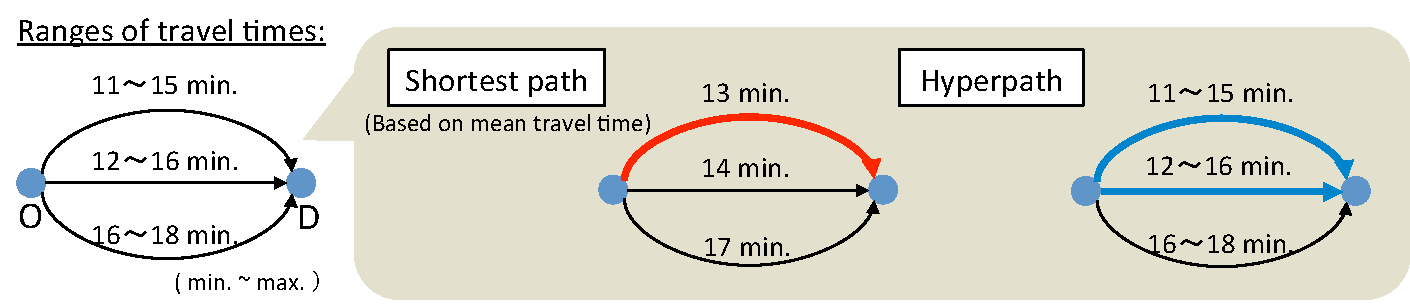
\includegraphics[width=0.90\textwidth, angle=0]{./scenarios/figures/tokyo_fig1.pdf}}%
{}
%------------

Hyperpath-based navigation can be beneficial in at least three ways: 
\begin{enumerate}
\item The concept of hyperpath could benefit drivers by helping reduce travel time unreliability; it provides an 'adaptive choice opportunity' to potentially avoid stops at intersections, or long delays on links. For example, other than typical navigation systems, the turn notification received by drivers before entering intersections could be ``go straight or turn right''. In this case, drivers may decide to turn right when encountering a red light for going straight. Even if the final experienced travel time is slightly longer than the non-adaptive drive, driving experience could be better (say, eight\,minutes driving plus two\,minutes waiting versus ten\,minutes non-stop driving).
\item For drivers, hyperpath also could cater more to individual tastes without pre-defining drivers' actual route choice preferences. Comparatively, shortest path (SP), or multiple shortest paths with different criterion, would require modelers' definition of ``shortest''. In the long run, the hyperpath model has the potential to evolve with reinforcement learning technologies and provide more customized adaptive route guidance.
\item Existing commercial navigation systems seldom take their effect on networks into consideration; sometimes congestion is actually produced by navigation systems. Thus, \gls{dta}, along with route guidance, might be still be mostly academic or hypothetical. Classical \gls{dta} are largely based on time-dependent K-shortest paths and aim to analyze equilibrium conditions as ideal states. For example, Dynamic User Equilibrium defines the equilibrium where drivers cannot change their trip plans to reduce actual experienced travel time. However, experienced travel time can never be known beforehand, since real-life transportation is much more complicated than laboratory \gls{dta} settings. Hyperpath-based route choice does not search for equilibrium, but it might be equilibrium-like to some extent, as it is strategically reactive to delay changes. 
\end{enumerate}

The hyperpath-based route recommendation could thus reduce overall network congestion, because it recommends a potential optimal set of paths instead of the shortest (single) path and leads to appropriate dispersion of traffic. However, its impact on the entire traffic networks has not been well analyzed. In this chapter, we demonstrate---using \gls{matsim}---how hyperpath-based vehicle navigation market penetration would affect overall network performance.  Though development of real-time traffic information for navigating vehicles has benefited drivers, to some extent, market diffusion of these technologies may not lead to the reduction of traffic congestion, mainly due to the concentration of traffic into particular paths or links in the traffic networks. Certain unexpected phenomena, such as ``Hunting \citep[e.g.,][]{Oguchi2003}'', might occur. We changed the ratio of vehicles with risk-averse route guidance, conducted traffic simulation and then checked traffic performance.


\section{A Small-Sized Network Case}

\gls{matsim} was utilized as the simulation tool. In the early stage, we conducted such simulations on the Sioux Falls network (see also Chapter~\ref{ch:siouxfalls}) with synthetic \gls{od} demands (see \citep{Yamada2013} for details). Hyperpath algorithm was initially written as an external route planning module in Python and the market share can be configured by setting the ``ModuleProbability'' item. Figure~\ref{fig:tokyo_fig2} illustrates the configuration sample for hyperpath with 20\,\% market share. Figure~\ref{fig:tokyo_fig3} also shows the network state (in terms of link speed) improvement with increase in the market share of hyperpath from 20\,\% to 80\,\%.

%------------
\createfigure%
{Setting for the case that 20 \% of vehicles follow hyperpath-based vehicle navigation}%
{Setting for the case that 20 \% of vehicles follow hyperpath-based vehicle navigation}%
{\label{fig:tokyo_fig2}}%
{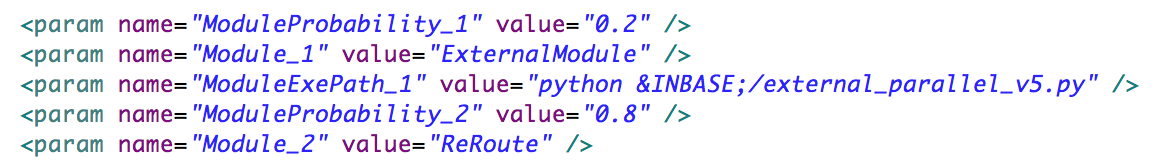
\includegraphics[width=0.95\textwidth, angle=0]{./scenarios/figures/tokyo_fig2.png}}%
{}
%------------

%------------
\createfigure%
{Link travel speeds for different levels of market penetrations}%
{Link travel speeds for different levels of market penetrations}%
{\label{fig:tokyo_fig3}}%
{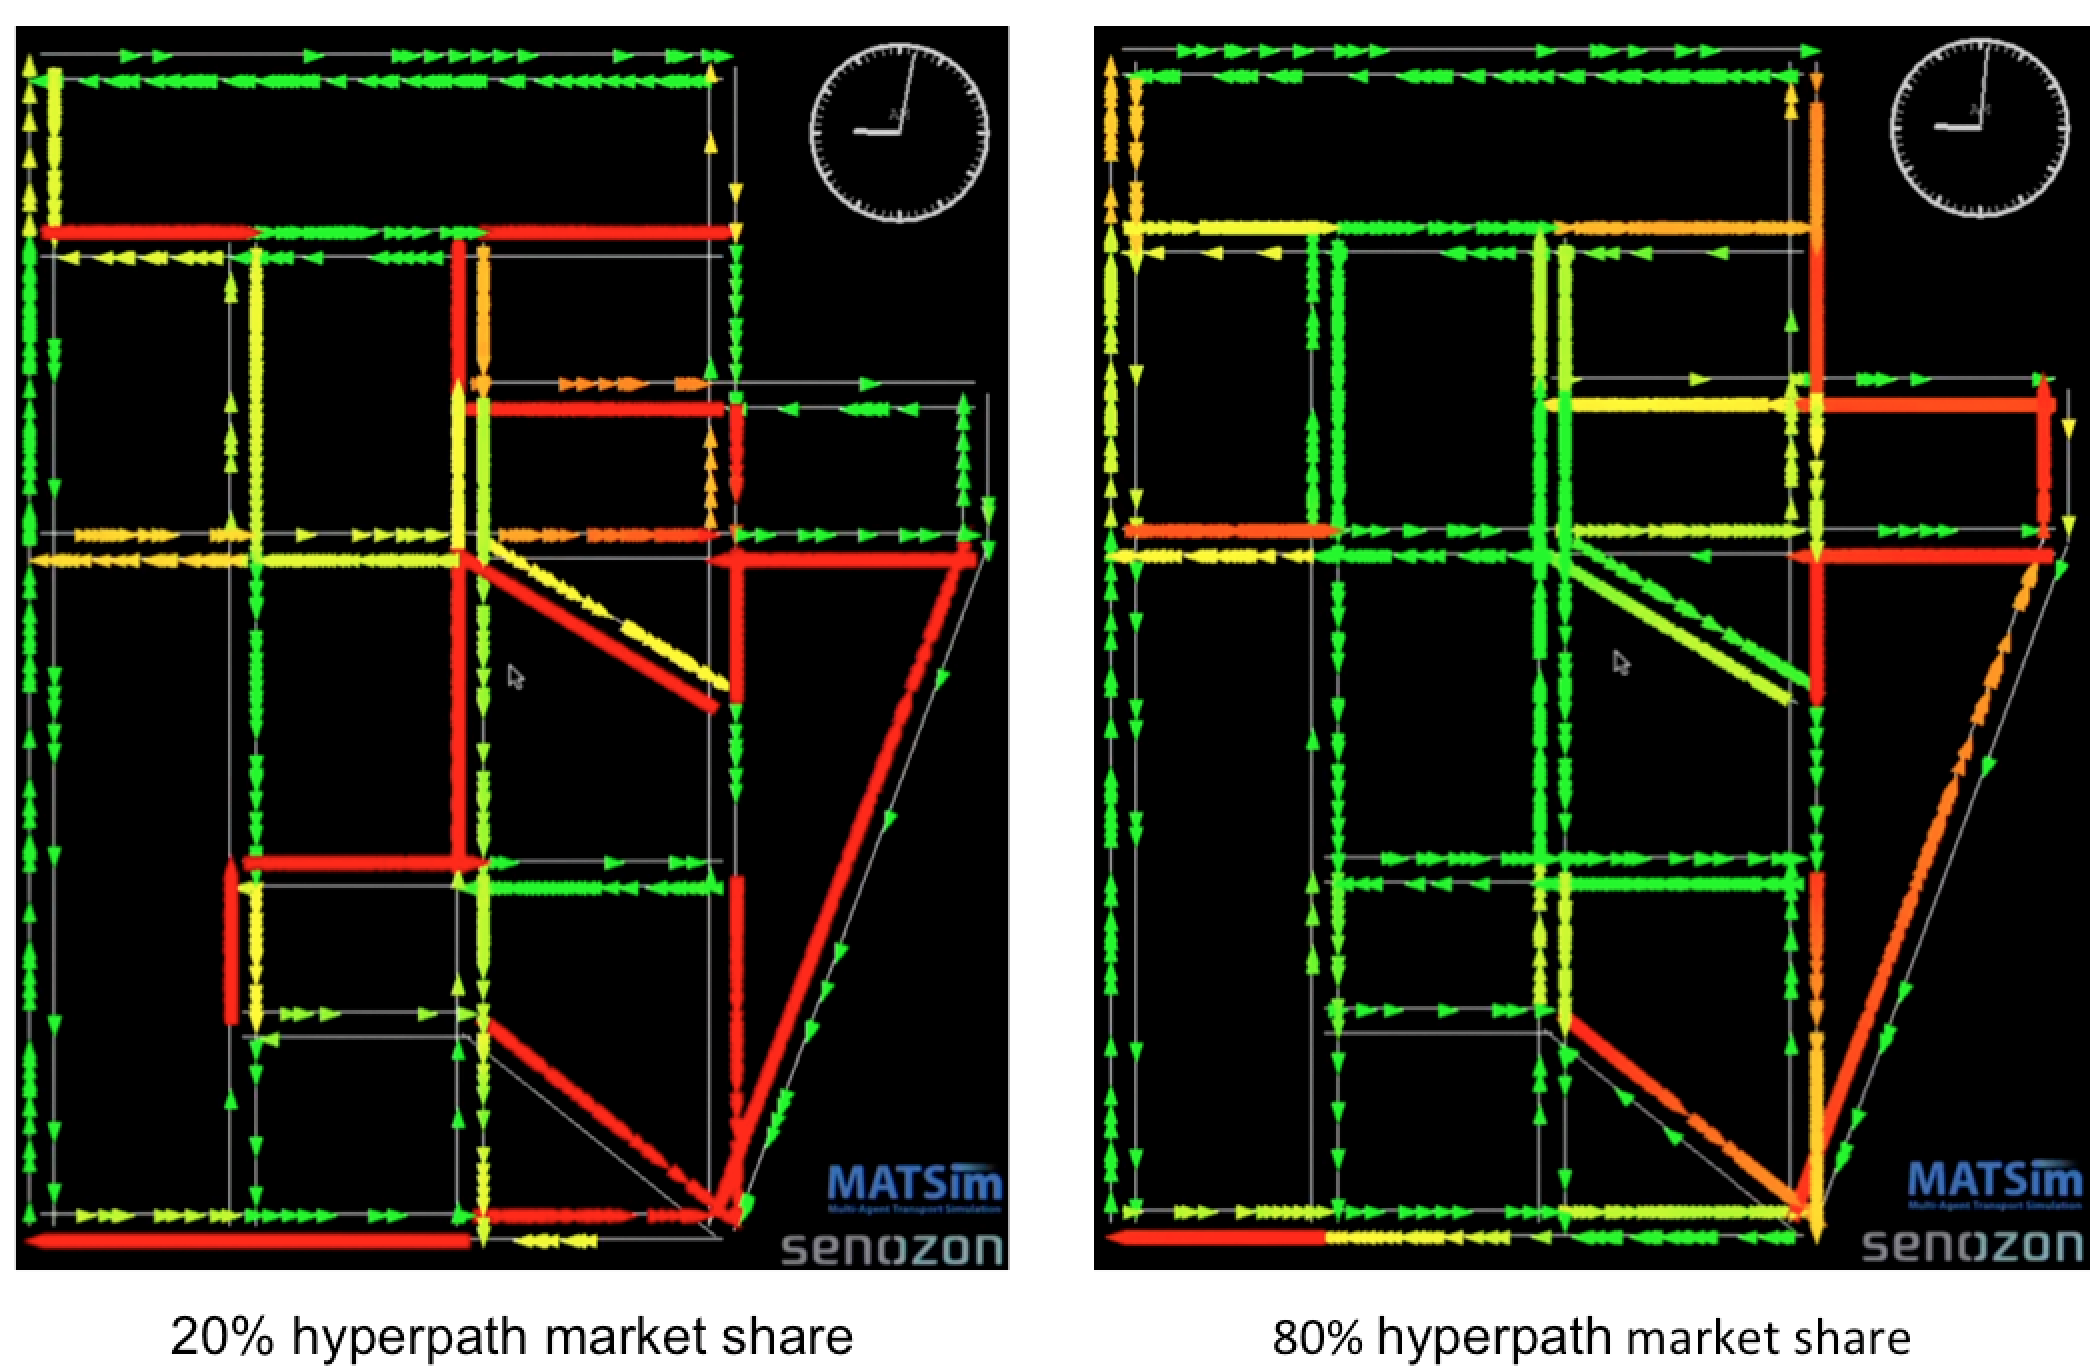
\includegraphics[width=0.85\textwidth, angle=0]{./scenarios/figures/tokyo_fig3.png}}%
{}
%------------


\section{Simulation in Tokyo's Arterial Road Network}
Based on early-stage experiments on the Sioux Falls network, we were interested in a similar simulation in Tokyo's large-scale arterial network with actual traffic data. 

\subsection{Network and Travel Demand}
The arterial road network, including the whole Tokyo Metropolitan Area (Figure~\ref{fig:tokyo_fig4}), was prepared from Digital Road Map version~2011 (DRM2403) in a radius of about 70--80\,kilometer from downtown. The traffic network consisted of 444\,220\,nodes and 177\,971\,links after being cleaned using the ``networkcleaner'' API in \gls{matsim}. Capacity and free flow speed of each link were set up considering road hierarchy information, type of links and their corresponding speed limits. 

 %------------
\createfigure%
{Arterial road network in Tokyo Metropolitan Area}%
{Arterial road network in Tokyo Metropolitan Area}%
{\label{fig:tokyo_fig4}}%
{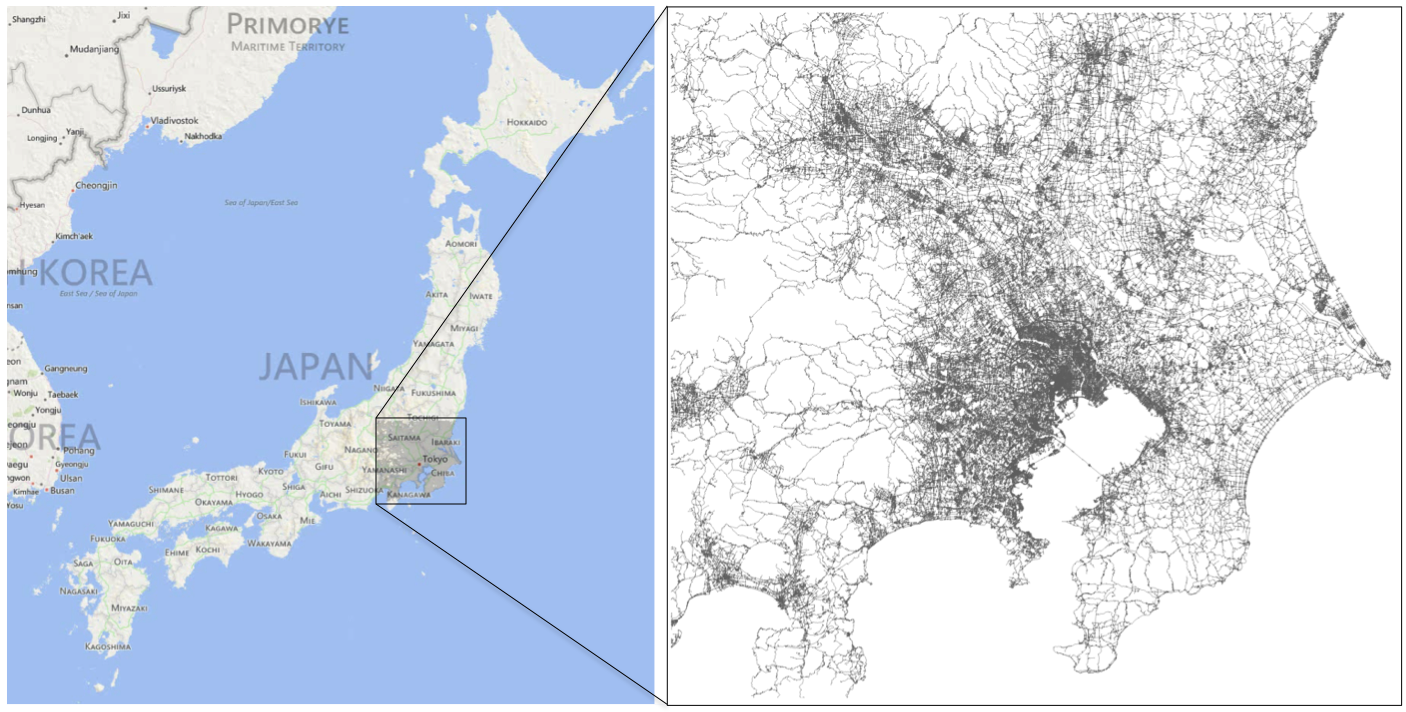
\includegraphics[width=0.90\textwidth, angle=0]{./scenarios/figures/tokyo_fig4.png}}%
{}
 %------------

We analyzed car traffic during morning rush hours and the \gls{od} table was subtracted from a large-scale travel survey (Person Trip Survey~2007) to create agents' plans. The total number of the \gls{od} pairs was 17\,186 and there were about 2\,307\,000 vehicular trips during the target time period within the whole area. From the data, 219\,642 agents (approximately 10\,\% sampling rate) were randomly created and each agent had only one activity, commuting from his/her home to the workplace. For drivers' departure time from home, a normal distribution with the mean of 7\,AM and the standard deviation of 1\,hour was assumed.

\subsection{Setup of Day-to-Day Simulation Experiments}
Although the Logit-based route planning module had already been employed as one of the \gls{matsim} routing strategies, it may have had less supportive route guidance explanations. We thus focused on the combination of ``re-route'' and ``best-score'' planning modules, which meant that some drivers adjusted their daily travel plan according to yesterday's experience, while the others simply chose the most positive route from their past choices. 

To get travel time data for creating hyperpaths, simulation runs for 30\,iterations (\ie 30\,days) were firstly performed with no HP-based drivers (\ie 100\,\% of SP-based drivers) to obtain travel time distribution. Then, maximum delays in each during these 30\,days were computed and used in the following main simulation, with the market diffusion of HP-based navigated drivers. Figure~\ref{fig:tokyo_fig5} illustrates a simulation with \gls{matsim} for the downtown Tokyo. 

%------------
\createfigure%
{Snapshot of the hyperpath-based traffic simulation in Tokyo}%
{Snapshot of the hyperpath-based traffic simulation in Tokyo}%
{\label{fig:tokyo_fig5}}%
{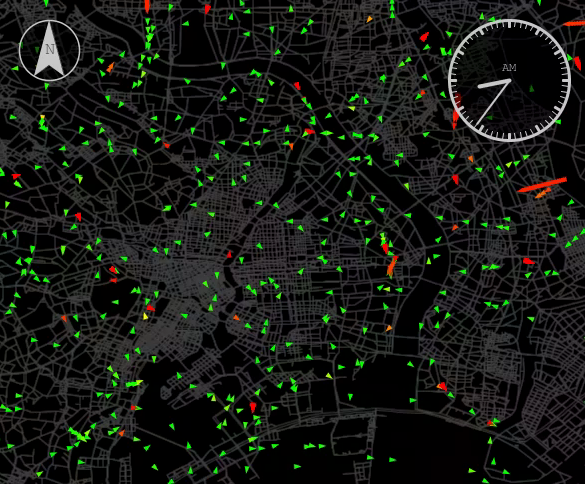
\includegraphics[width=0.68\textwidth, angle=0]{./scenarios/figures/tokyo_fig5.png}}%
{}
 %------------

\subsection{Results}
We conducted five different cases of traffic simulation by changing the shares of HP-based drivers from 0\% to 80\% by 20\%. The simulation runs were conducted for 30\,days for each case to evaluate network-level travel-time savings, as well as reliability. 

Average travel time per unit length of all agents in each one day was plotted for different cases in Figure~\ref{fig:tokyo_fig6}. Since the traffic network in Tokyo is quite large and drivers' trip lengths are diverse, we plotted the average travel time per unit length (shortly ATTPUL) for a fair comparison. Apparently, there were high levels and large fluctuations in ATTPUL when there were no HP-based drivers (HP\,\%, that is SP 100\,\%). But it is obvious that, as the market diffusion rate of HP-based drivers increased, fluctuation and levels of ATTPUL  would be significantly reduced.


%------------
\createfigure%
{Average travel time per unit length for all vehicles}%
{Average travel time per unit length for all vehicles}%
{\label{fig:tokyo_fig6}}%
{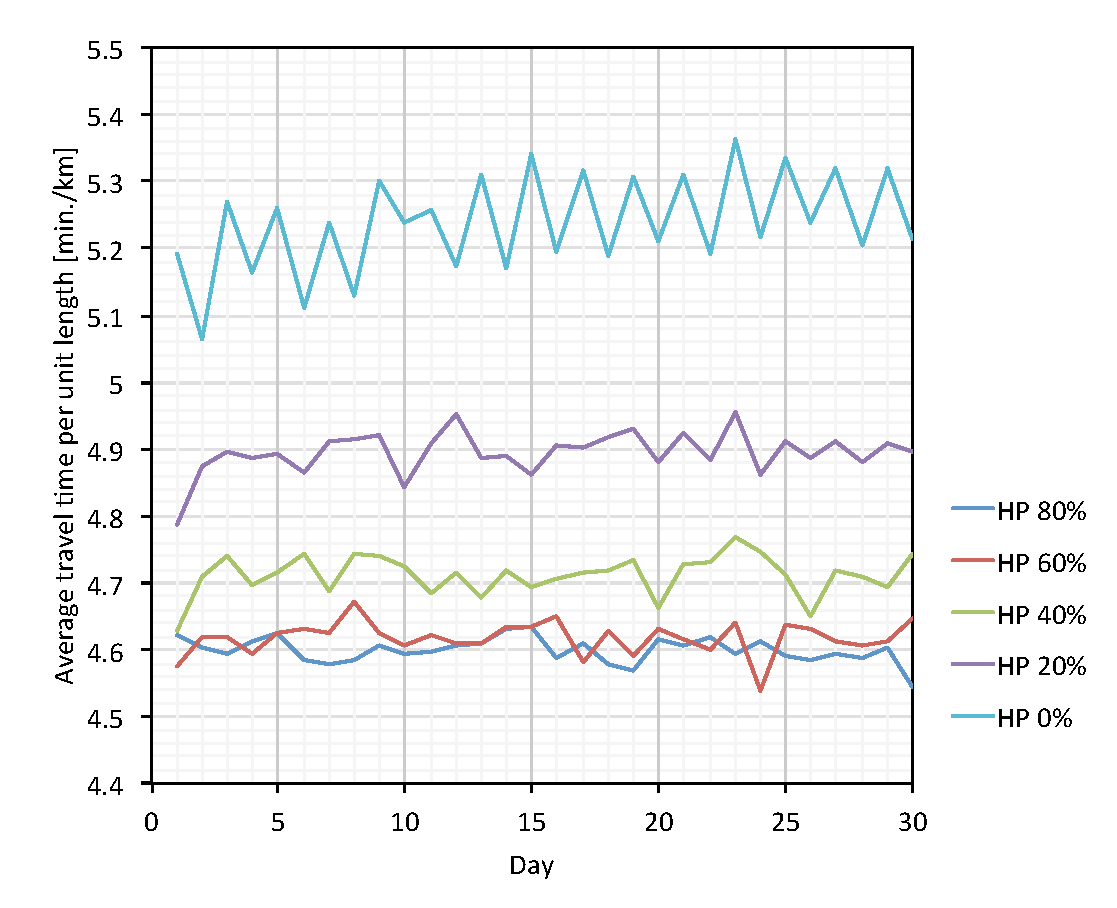
\includegraphics[width=0.70\textwidth, angle=0]{./scenarios/figures/tokyo_fig6.pdf}}%
{}
 %------------


Table~\ref{tab:tokyo_1} summarizes the result of Figure~\ref{fig:tokyo_fig6} by computing the ATTPUL ($\overline{t}_{unit}$) average, as well as the ATTPUL ($\sigma_{unit}$) standard deviation over the 30\,days. It is clear from this table that both average and standard deviation of travel time tended to decrease when the mixing ratio of HP-based route guidance was increased. This result indicates that HP-based route guidance would be superior in terms of of travel time reduction and reliability given day-to-day patterns of average travel time for  heavy Tokyo traffic. 

\createtable%
	{Summary of the network perfomance}%
	{Summary of the network perfomance}%
	{\label{tab:tokyo_1}}%
	{%
	\begin{tabular}{ccc}
	\hline
			Case & $\overline{t}_{unit}$ [min./km] & $\sigma_{unit}$ [min./km]\\
			\hline
			HP 80\%& 4.60& 0.02 \\
			HP 60\%& 4.62 & 0.02 \\
			HP 40\%& 4.71 & 0.03 \\
			HP 20\%& 4.90 & 0.03  \\
			HP 0\%& 5.24 & 0.07 \\
			\hline
\end{tabular}
}%
{}%

\section{Validation of Hyperpath-Based Navigation}
A field experiment was conducted to verify the benefits of travel time reliability improvement for drivers by \citet{Ito2015} in Tokyo. Drivers equipped with the time-dependent shortest path and those equipped with the time-dependent hyperpath navigation systems were compared. Both navigation systems use the same historical travel time sourced from probe vehicle data. Based on results collected from two weeks of experimental driving by different drivers, the hyperpath produced a significantly better result, especially when the network was congested. 

% ##################################################################################################################